\documentclass{beamer}
\usetheme{Boadilla}
\mode<presentation>

\title{The Transfer Matrix Method in Linear Dielectrics}
\author{Claudio Barros}
\institute{University at Buffalo}
\date{\today}

\begin{document}
	

	


	
\begin{frame}
	
\titlepage

\end{frame}







\begin{frame}
	
\frametitle{Outline}

\tableofcontents

\end{frame}






\section{Electromagnetic Plane-Waves in Dielectric Media}

\section{Reflection and Transmission at Dielectric Interfaces}

\section{The Transfer Matrix Method}






\begin{frame}

	
	
\frametitle{Electromagnetic Plane-Waves in Dielectric Media}



As always, our starting point is the Maxwell equations: 
\begin{equation}
	\nabla \cdot \mathbf{D} = \rho_{f}
\end{equation}
\begin{equation}
	\nabla \cdot \mathbf{B} = 0
\end{equation}
\begin{equation}\label{faraday}
	\nabla \times \mathbf{E} = - \frac{\partial \mathbf{B}}{\partial t}
\end{equation}
\begin{equation}\label{ampere}
	\nabla \times \mathbf{H} =  \frac{\partial \mathbf{D}}{\partial t} + \mathbf{J}_{f}
\end{equation}
In the case of linear and isotropic media we have the following relations for our fields:
\begin{equation}
	\mathbf{D} = \epsilon \mathbf{E}
\end{equation}
\begin{equation}
	\mathbf{H} = \frac{1}{\mu} \mathbf{B}
\end{equation}



\end{frame}






\begin{frame}



In the absence of any sources, the Maxwell equations can be combined to obtain the Helmholtz equations: 			
\begin{equation}\label{helm1}
	(\nabla^{2} + \mu \epsilon \omega^{2}) \mathbf{E} = 0
\end{equation}
\begin{equation}\label{helm2}
	(\nabla^{2} + \mu \epsilon \omega^{2}) \mathbf{B} = 0
\end{equation}
The solutions? Plane-waves, of course!
\begin{equation}
	\mathbf{E}(\mathbf{r}, t) = \mathbf{E}_{0} e^{i( k \mathbf{n} \cdot \mathbf{r} - \omega t )}
\end{equation}
\begin{equation}
	\mathbf{B}(\mathbf{r}, t) = \mathbf{B}_{0} e^{i( k \mathbf{n} \cdot \mathbf{r} - \omega t )}
\end{equation}
The dispersion relation and index of refraction can also be obtained now:
\begin{equation}
	k^{2} = \mu \epsilon \omega^{2}
\end{equation}
\begin{equation}\label{index}
	n = \sqrt{ \frac{ \mu \epsilon }{ \mu_{0} \epsilon_{0} } }
\end{equation}



\end{frame}






\begin{frame}
	
	
	
\frametitle{Reflection and Transmission at Dielectric Interfaces}



\begin{figure}[h]
	\centering
	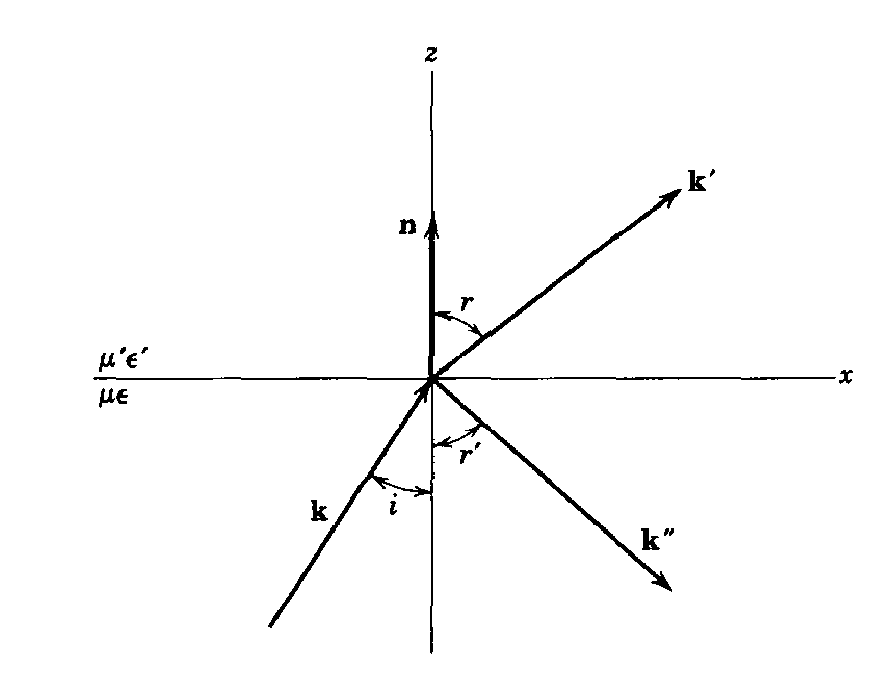
\includegraphics[width=.65\linewidth]{1}
	\caption{Propagation of a wave into a medium with a different index of refraction, which gives rise to reflected and refracted waves. The y-axis points into the page for this geometry [\textbf{1}].}
	\label{fig:lat}
\end{figure}	



\end{frame}






\begin{frame}
	
	

We can join all three waves at the interface and use the superposition principle:	
\begin{equation}\label{superp}
	\mathbf{E}_{0} e^{i (\mathbf{k} \cdot \mathbf{r} - \omega t)} + \mathbf{E}_{0}'' e^{i (\mathbf{k}'' \cdot \mathbf{r} - \omega t)} = \mathbf{E}_{0}' e^{i (\mathbf{k}' \cdot \mathbf{r} - \omega t)}
\end{equation}
\begin{equation}\label{k1}
	|\mathbf{k}| = |\mathbf{k}''| = \omega \sqrt{\mu \epsilon}
\end{equation}
\begin{equation}\label{k2}
	|\mathbf{k}'| = \omega \sqrt{\mu' \epsilon'}
\end{equation}
\begin{equation}
	\mathbf{k} \cdot \mathbf{r} =  \mathbf{k}'' \cdot \mathbf{r} = \mathbf{k}' \cdot \mathbf{r}
\end{equation}
The laws of reflection and refraction then come out as natural consequences:
\begin{equation}
	|k||r| \cos \theta_{i} = |k''||r| \cos \theta_{r'} \hspace{10mm} \rightarrow \hspace{10mm}\theta_{i} = \theta_{r'}
\end{equation}
\begin{equation}
	k \sin \theta_{i} = k' \sin \theta_{r}
\end{equation} 



\end{frame}






\begin{frame}
	
	
	
The dynamic properties are a direct result of the boundary conditions at the dielectric interface:	
\begin{equation}
	[ \epsilon (\mathbf{E}_{0} + \mathbf{E}_{0}'') - \epsilon' \mathbf{E}_{0}' ] \cdot \mathbf{n} = 0
\end{equation}
\begin{equation}
	[ \mathbf{k} \times \mathbf{E}_{0} + \mathbf{k}'' \times \mathbf{E}_{0}'' - \mathbf{k}' \times \mathbf{E}_{0}' ] \cdot \mathbf{n} = 0
\end{equation}
\begin{equation}
	(\mathbf{E}_{0} + \mathbf{E}_{0}'' - \mathbf{E}_{0}' ) \times \mathbf{n} = 0
\end{equation}
\begin{equation}
	\left[ \frac{1}{\mu} ( \mathbf{k} \times \mathbf{E}_{0} + \mathbf{k}'' \times \mathbf{E}_{0}'' ) - \frac{1}{\mu'} ( \mathbf{k}' \times \mathbf{E}_{0}') \right] \times \mathbf{n} = 0
\end{equation}

	
	
\end{frame}





	
\begin{frame}
	
	

The the key outcome is the acquisition of the Fresnel equations: 
\begin{equation}\label{fresnel1}
	r_{p} = \frac{ n_{f} \cos \theta_{i} - n_{i} \cos \theta_{f} }{ n_{f} \cos \theta_{i} + n_{i} \cos \theta_{f}}
\end{equation}
\begin{equation}
	t_{p} = \frac{ 2 n_{i} \cos \theta_{i} }{ n_{f} \cos \theta_{i} + n_{i} \cos \theta_{f}}
\end{equation}
\begin{equation}
	r_{s} = \frac{ n_{i} \cos \theta_{i} - n_{f} \cos \theta_{f} }{ n_{i} \cos \theta_{i} + n_{f} \cos \theta_{f}}
\end{equation}
\begin{equation}\label{fresnel2}
	t_{s} = \frac{ 2 n_{i} \cos \theta_{i} }{ n_{i} \cos \theta_{i} + n_{f} \cos \theta_{f}}
\end{equation}



\end{frame}	






\begin{frame}
	
	
	
\frametitle{The Transfer Matrix Method}



We imagine a stacked layer of dielectric slabs with different properties:
\begin{align}\label{layers}
	n(z) =& n_{0}, \hspace{10mm} z < z_{0}                  \nonumber \\
	& n_{1}, \hspace{10mm} z_{0} < z < z_{1}           \nonumber \\
	& n_{2}, \hspace{10mm} z_{1} < z < z_{2}            \nonumber \\
	& \vdots                                             \nonumber \\ 	
	& n_{N}, \hspace{10mm} z_{N - 1} < z                  \nonumber \\	 
\end{align}
Note that $n$ is a function of $z$.



\end{frame}






\begin{frame}



Lets examine the relation between forward and backward E-fields in two different layers:
\begin{align}\label{system2}
	E_{F}' = E_{F} e^{ i k_{zj} z }  \nonumber \\
	E_{B}' = E_{B} e^{ -i  k_{zj} z }
\end{align}
Looks a lot like a matrix equation...
\begin{equation}
	E' = T_{j} E
\end{equation}
The two transfer matrices are then:
\begin{equation}\label{Tj}
	T_{j} = 
	\begin{pmatrix}
		\exp i \Phi_{j} & 0 \\
		0 & \exp - i \Phi_{j}
	\end{pmatrix}
\end{equation}
\begin{equation}\label{Tji}
	T_{ji} = \frac{1}{t_{ji}}
	\begin{pmatrix}
		1 & r_{ji} \\
		r_{ji} & 1
	\end{pmatrix}
\end{equation}
Whereas the \textit{full} transfer matrix becomes:
\begin{equation}
	T = T_{N(N-1)} T_{N-1} \hdots T_{32} \hspace{1mm} T_{2} \hspace{1mm} T_{21} \hspace{1mm} T_{1} \hspace{1mm} T_{10}
\end{equation}



\end{frame}






\begin{frame}



Finally, our desired results! 
\begin{equation}
	R = |r|^{2}
\end{equation}
\begin{equation}
	T_{p} = |t|^{2} \frac{  \mathrm{Re} ( n_{f} \cos \theta_{f}^{*} )  }{ \mathrm{Re} ( n_{i} \cos \theta_{i}^{*}  ) }
\end{equation}
\begin{equation}
	T_{s} = |t|^{2} \frac{  \mathrm{Re} ( n_{f} \cos \theta_{f} )  }{ \mathrm{Re} ( n_{i} \cos \theta_{i} ) }
\end{equation}



\end{frame}






\begin{frame}


\frametitle{References}


\begin{thebibliography}{1}
	
\bibitem{1} J. Jackson, \textit{Classical Electrodynamics} (John Wiley \& Sons, Inc., 1999).
	
\bibitem{2} E. Hecht, \textit{Optics} (Pearson, 2002).
	
\bibitem{3} M. Born, and E. Wolf, \textit{Priciples of Optics} (Pergamon Press, 1986).
	
\bibitem{4} M. Claudia Troparevsky, Adrian S. Sabau, Andrew R. Lupini, and Zhenyu Zhang, "Transfer-matrix formalism for the calculation of optical response in multilayer systems: from coherent to incoherent interference," Opt. Express 18, 24715-24721 (2010)
	
\bibitem{5} https://pypi.org/project/tmm/
	
\end{thebibliography}



\end{frame}






\end{document}
